Overall, using TA to collect data for the UCB1-AKSB algorithm was a success. Not only did the site facilitate over 8,000 online conversations among Princeton students, but it also gained significant traction on campus. From its initial launch, Tigers Anonymous had over 40,000 page-views and over 6,000 unique visitors (see \autoref{fig:GoogleAnalytics} for the full Google Analytics dashboard). Over time, TA's daily usage stabilized to relatively modest levels, most likely because of user stratification and/or saturation, which is explored in further detail in \autoref{sec:IndividualUserAnalysis}.

\begin{figure}[H]
\centering
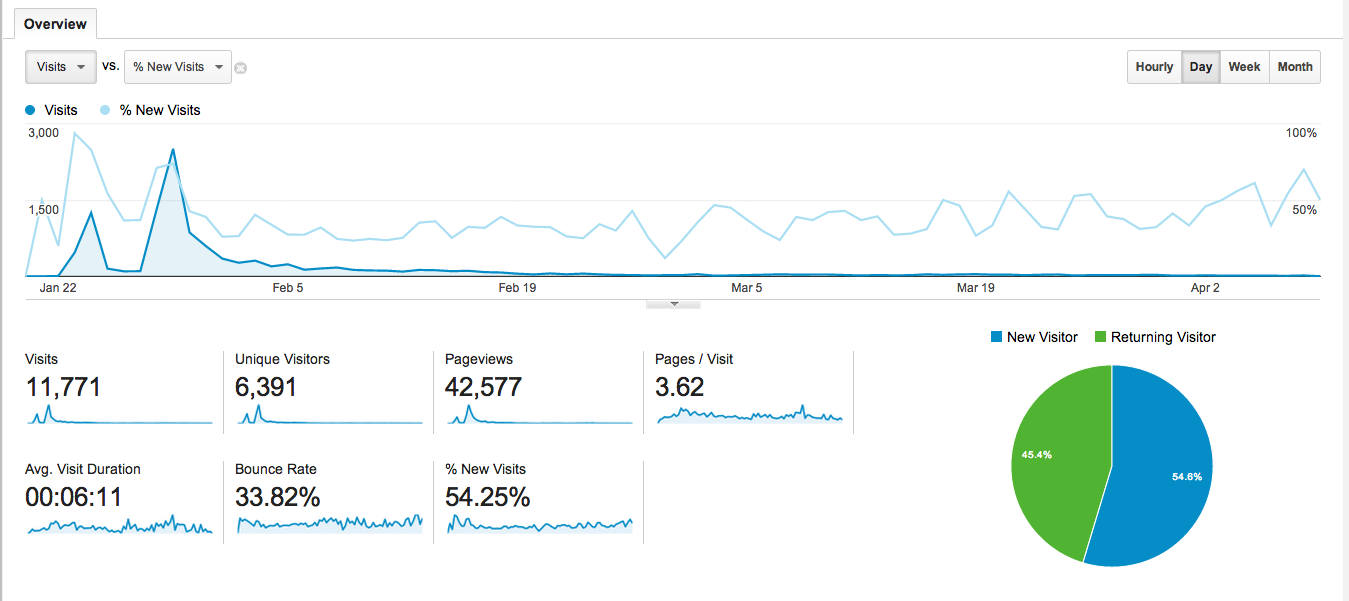
\includegraphics[trim= 0mm 0mm 0mm 0mm, clip, scale=0.3]{./Figures/GoogleAnalytics}
\caption{TA Google Analytics Dashboard}
\label{fig:GoogleAnalytics}
\end{figure}

\section{Regret Analysis}
\label{sec:RegretAnalysis}

Recall from \autoref{ch:LiteratureReview} that the cumulative regret of the UCB1 algorithm is proportional to log($n$), where $n$ is the number of plays. Thus, we should expect the UCB1-AKSB algorithm to result in a cumulative pseudo-regret that is approximately logarithmic in the number of plays. This empirical pseudo-regret, $\hat{R}_n$, was calculated using \autoref{eq:RegretComputation} below under the assumption that the long-term average de-anonymization rate ($\mu^{*}$) is optimal.

\begin{equation}
\label{eq:RegretComputation}
\hat{R}_n = \mu^{*}n - \sum_{t=1}^{n}{X_{I_t, t}}
\end{equation}

In \autoref{eq:RegretComputation}, $\mu^{*}n$ is the expected optimal number of de-anonymizations by play $n$ (i.e. $\max_{i=1,...,K}{\mathbb{E}\left[\sum_{t=1}^{n}{X_{i, t}}\right]}$ from \autoref{eq:PseudoRegret}). The plot of $\hat{R}_n$ as a function of $n$ for the UCB1-AKSB algorithm is shown below in \autoref{fig:TADe-AnonymizationRegret}.

\begin{figure}[H]
\centering
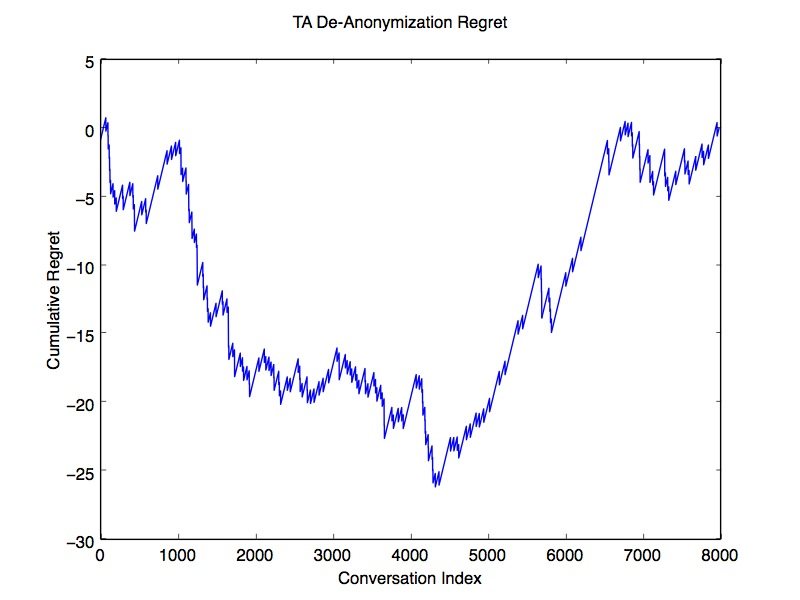
\includegraphics[trim= 0mm 0mm 0mm 0mm, clip, scale=0.5]{./Figures/TADe-AnonymizationRegret.jpg}
\caption{TA De-Anonymization Regret Analysis}
\label{fig:TADe-AnonymizationRegret}
\end{figure}

The regret looks approximately logarithmic for the second half of the dataset, but the first half of the data gives a steadily negative cumulative regret. This is because the assumption that conversation de-anonymization is IID is most likely false. Instead, there were probably different regimes in which people perceived Facebook de-anonymization differently. This is most analogous to the Markovian bandits in \cite{bubeck12}, where each conversation starter is associated with a Markov process with a discrete set of reward distributions.

Because of the clear split in the data, it seems that there were two discrete distributions from which de-anonymizations were drawn. The first distribution occurred in the initial stages of TA's launch, where users were more likely to have long conversations and de-anonymize the conversation simply because of the novelty of doing so. This is supported by looking at the initial cumulative Facebook de-anonymization statistics (see \autoref{fig:TADe-AnonymizationCumulative}), where the Facebook connect rate was almost double the long-term average. The second distribution most likely occurred as the novelty of de-anonymization wore off and users opted for de-anonymization only if the conversation was of sufficiently high quality. The existence of multiple regimes explains the two parts of the regret data in \autoref{fig:TADe-AnonymizationRegret}.

However, the second part of the cumulative regret plot in \autoref{fig:TADe-AnonymizationRegret} still looks logarithmic, which suggests that the algorithm performed in-line with expectations during the second regime of TA usage.

\begin{figure}[H]
\centering
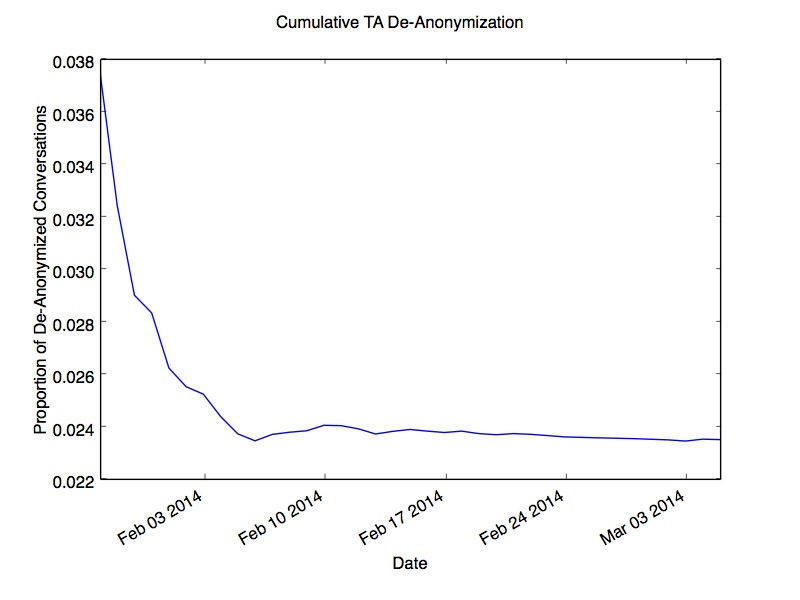
\includegraphics[trim= 0mm 0mm 0mm 0mm, clip, scale=0.5]{./Figures/CumulativeTADe-Anonymization.jpg}
\caption{TA Cumulative Conversation De-Anonymization Rate}
\label{fig:TADe-AnonymizationCumulative}
\end{figure}

\section{UCB1-AKSB Effectiveness}

Since conversation de-anonymization was the metric that UCB1-AKSB used to judge each conversation starter, the obvious way to measure the performance of the UCB1-AKSB algorithm is to observe the proportion of conversations which were de-anonymized. Judging from not only the cumulative de-anonymization proportion (\autoref{fig:TADe-AnonymizationCumulative}) but also the daily de-anonymization proportion (\autoref{fig:TADe-AnonymizationDaily}), it seems that the algorithm had little impact on whether or not people opted to de-anonymize the conversation. If anything, it looks like the algorithm had an adverse impact on conversation de-anonymization.

However, this may have been due to the fact that the user's decision to de-anonymize the conversation was based on factors other than the conversation starter. It is easy to imagine an anonymous conversation which became extremely personal and users were therefore hesitant to reveal their identities in fear of being connected to the conversation. In such cases, the conversation starter may have been excellent but the conversational and/or social tendencies of the users would prevent them from de-anonymizing. In other words, the process of conversation de-anonymization may be more user-specific than assumed by the UCB1-AKSB algorithm. This, in turn, could have resulted in a downward drag on overall de-anonymization rates even as the conversation starter quality improved.

Additionally, recall that the option to de-anonymize a conversation only came after both users had exchanged a pre-specified number of messages (in the current implementation, this number is 15). The implication is clear: it is possible that many of these conversations never even had the opportunity to de-anonymize, so marking them as `failures' in the data model is misleading. This claim is empirically validated by aggregate TA user data as shown in \autoref{fig:UCBSavingGrace}. 

\begin{figure}[H]
\centering
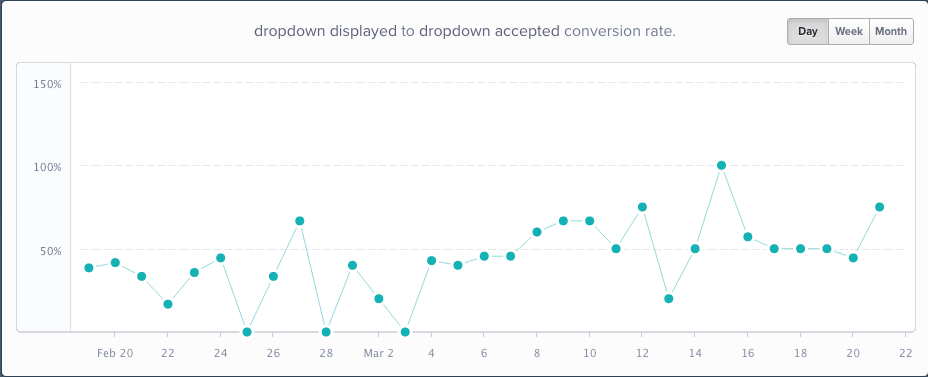
\includegraphics[trim= 1mm 1mm 0mm 1mm, clip, scale=0.45]{./Figures/UCBSavingGrace}
\caption{TA Conditional De-Anonymization Rate}
\label{fig:UCBSavingGrace}
\end{figure}

This plot shows that, after being given the option to de-anonymize, users gradually became more likely to do so. This suggests that the UCB1-AKSB algorithm was improving the quality of conversation starters despite the overall drop in de-anonymizations. In other words, even though the proportion of people who de-anonymized decreased slightly, the proportion of people who did so when given the opportunity actually increased, which suggests that UCB1-AKSB may have been at least moderately effective in spurring de-anonymization.

In any case, the metric of conversation de-anonymization itself introduces difficulties in accurately measuring incremental improvements in conversation quality. For example, let us say the conversation de-anonymization would only occur if the conversation `quality' metric were above some threshold $d$. Even if the UCB1-AKSB algorithm boosted the quality of otherwise low-quality conversation by providing some common ground, such a quality boost would not be visible unless the incremental improvement was enough to make such conversations pass the threshold $d$. Basically, it is entirely possible that the UCB1-AKSB algorithm could improve conversation quality but this increased likelihood would not be visible because of the censored data observed. This `censored-data' hypothesis would also explain some of the erratic behavior of the daily de-anonymization rate seen in \autoref{fig:TADe-AnonymizationDaily}.

\begin{figure}[H]
\centering
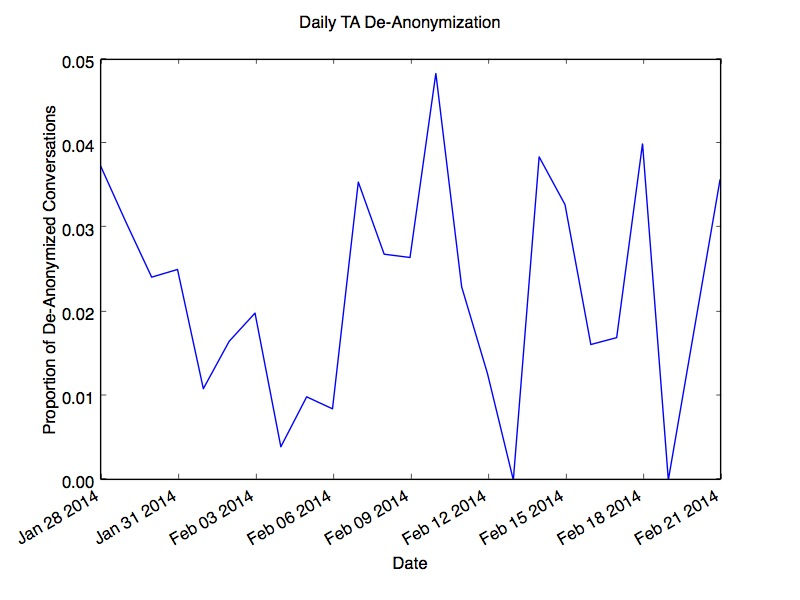
\includegraphics[trim= 0mm 0mm 0mm 0mm, clip, scale=0.5]{./Figures/DailyTADe-Anonymization.jpg}
\caption{TA Daily Conversation De-Anonymization Rate}
\label{fig:TADe-AnonymizationDaily}
\end{figure}

Given that conversation de-anonymization might have been affected by other exogenous variables and was not granular enough to measure incremental improvements in conversation quality, it makes sense to turn to other conversation quality metrics to judge the performance of UCB1-AKSB. These other metrics (participation rates and average conversation rates) are less likely to be influenced by the social pressure for or against de-anonymization, and have a more finely differentiated set of values than the binary variable of conversation de-anonymization. The plots of both these metrics are shown below in \autoref{fig:TAParticipationCumulative} and \autoref{fig:TAMessagesExchangedCumulative}.

\begin{figure}[H]
\centering
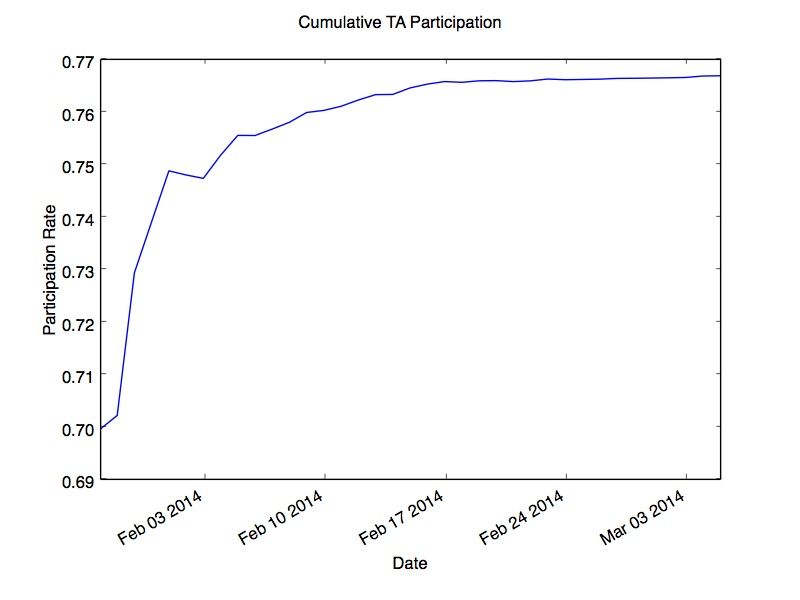
\includegraphics[trim= 0mm 0mm 0mm 0mm, clip, scale=0.5]{./Figures/CumulativeTAParticipation.jpg}
\caption{TA Cumulative Participation Rate}
\label{fig:TAParticipationCumulative}
\end{figure}

\begin{figure}[H]
\centering
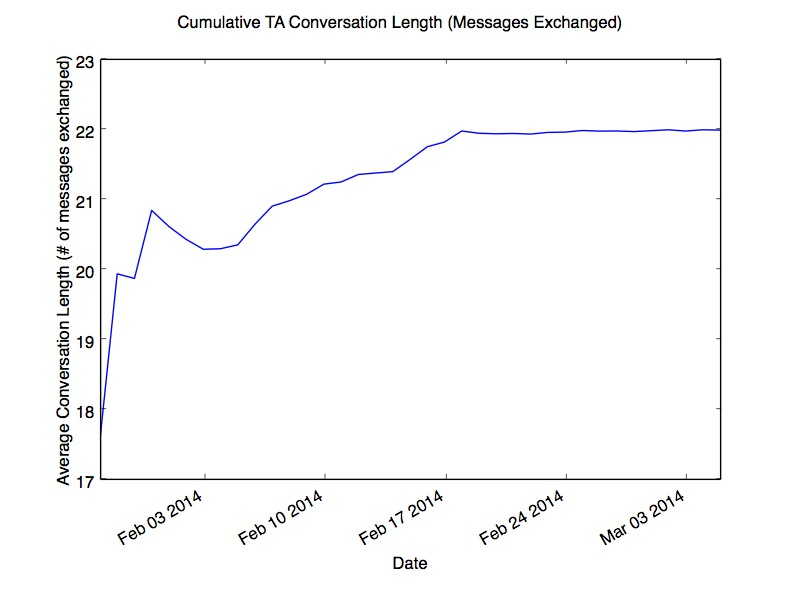
\includegraphics[trim= 0mm 0mm 0mm 0mm, clip, scale=0.5]{./Figures/CumulativeTAConversationLength(MessagesExchanged).jpg}
\caption{TA Cumulative Average Conversation Length}
\label{fig:TAMessagesExchangedCumulative}
\end{figure}

By these metrics, it seems that conversation quality improved noticeably over time, which suggests that the UCB1-AKSB algorithm may still have had a positive effect on conversation quality even though some of its fundamental assumptions were not true.

\section{Individual User Analysis}
\label{sec:IndividualUserAnalysis}

Another way of examining the data is to look at how individual users behaved as they continued to interact with the site. In each of the plots below, the x-axis represents the number of uses, while the y-axis represents the conditional mean of the metric over the set of users on the $n$-th use, given that they have used the site at least $n$ times. In order to define this more clearly, I introduce the following notation: let $f_k(u, n)$ give the value of conversational quality metric $k$ for user $u$ on their $n$-th visit and function $g(u)$ give the number of times user $u$ has visited the site. Let $U_n$ be the set $\{u | u \in {U}, g(u) \geq{n}\}$ (i.e. the set of users who have visited the site at least $n$ times). Then, the graphs below are plots of $y_k(n)$ for different conversational quality metrics $k$ with $y_k(n)$ defined in \autoref{eq:PerUserFormula}.

\begin{equation}
\label{eq:PerUserFormula}
y_k(n) = \frac{1}{|U_n|}\sum_{u \in U_n}{f_k(u, n)}
\end{equation}

\begin{figure}[H]
\centering
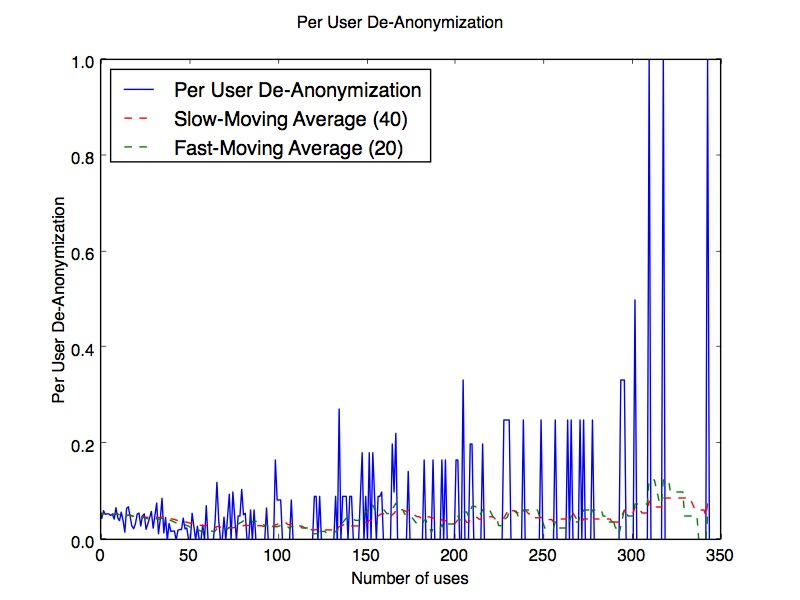
\includegraphics[trim= 0mm 0mm 0mm 0mm, clip, scale=0.5]{./Figures/PerUserDe-Anonymization.jpg}
\caption{De-Anonymization Rate Per User}
\label{fig:PerUserFBConnect}
\end{figure}

\begin{figure}[H]
\centering
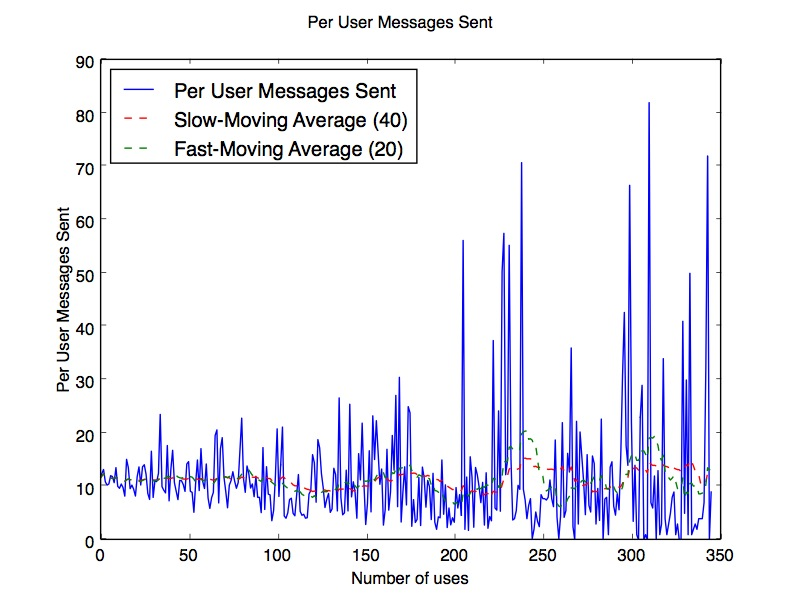
\includegraphics[trim= 0mm 0mm 0mm 0mm, clip, scale=0.5]{./Figures/PerUserMessagesSent.jpg}
\caption{Total Messages Sent Per User}
\label{fig:PerUserMessagesSent}
\end{figure}

\begin{figure}[H]
\centering
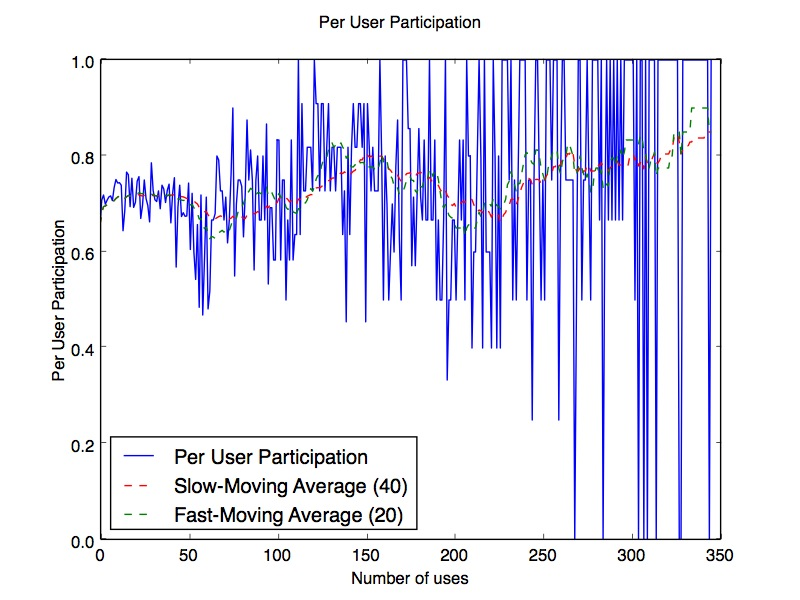
\includegraphics[trim= 0mm 0mm 0mm 0mm, clip, scale=0.5]{./Figures/PerUserParticipation.jpg}
\caption{Participation Rate Per User}
\label{fig:PerUserParticipation}
\end{figure}

The two things that immediately stand out from these plots are the general upward drift and the increasing volatility over time. The general upward drift of each conversation quality metric on a user-level supports the hypothesis that the UCB1-AKSB was increasing conversation quality over time. Another possible source of this upward drift is that users who visit the site frequently (who I will refer to as power-users) are more interested in having high-quality conversations and will seek to do so independently of the conversation starter. However, even if the latter hypothesis were true, the UCB1-AKSB algorithm still succeeded in providing a set of initial conversation starters to these users to make them power-users. Therefore, there is still evidence that the UCB1-AKSB algorithm was effective. Additionally, the steady increase in the conversation de-anonymization rate (\autoref{fig:PerUserFBConnect}) suggests that the algorithm actually performed quite well on a per-user basis, despite the modest cumulative de-anonymization performance (\autoref{fig:TADe-AnonymizationCumulative}).

On the other hand, the increasing volatility over time of each conversation quality metric represents the stratification of users into different classes. An abrupt change from a participation rate of 1.0 to 0.0 in one use in any of the above per-user plots is most likely the result of a power-user being paired with an amateur-user, which refers to someone who used TA very infrequently. In this case, the amateur-user would disconnect from the conversation before the power-user has a chance to participate meaningfully.

This user stratification is empirically validated by the behavior of TA users. For example, in \autoref{fig:UserStratificationVisitCount}, most of the visit density cluster in the 1-2 visit category and the 26-200 visit category. This bimodal distribution of user behavior is even more prevalent in \autoref{fig:UserStratificationVisitLength}, where the distribution is also clumped around short and long lengths of time spent on TA. This clearly supports the idea that, on both a amount-of-time and number-of-visits basis, TA users clumped into either power-users or amateur-users.

\begin{figure}[H]
\centering
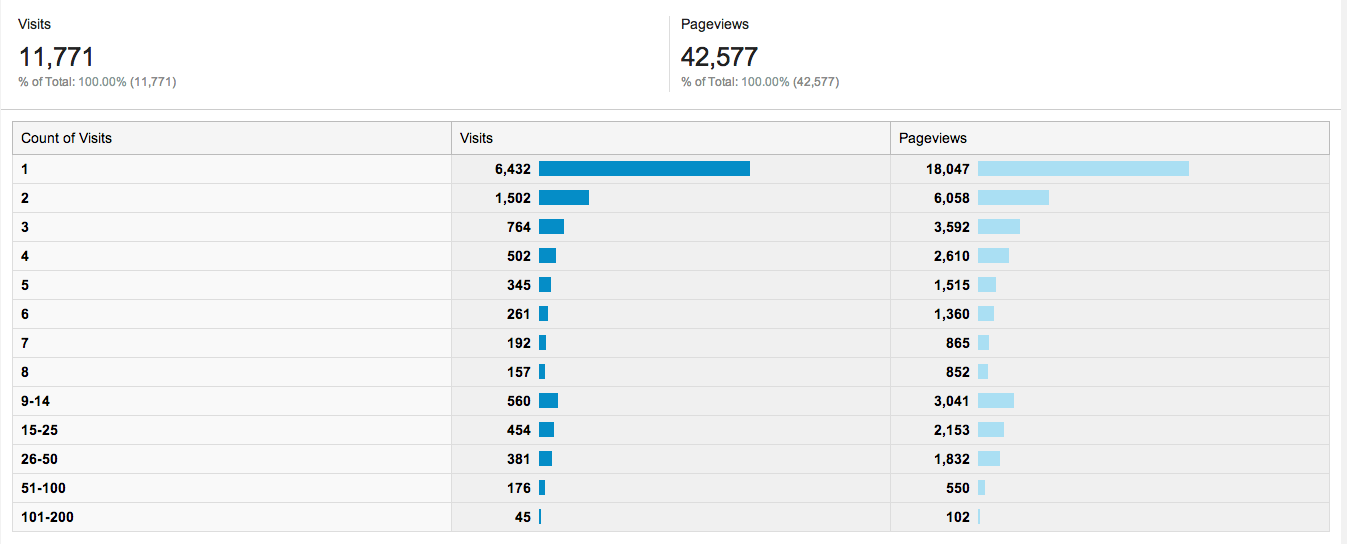
\includegraphics[trim= 0mm 0mm 0mm 0mm, clip, scale=0.3]{./Figures/UserStratificationVisitCount}
\caption{User Engagement by Visit Count}
\label{fig:UserStratificationVisitCount}
\end{figure}

\begin{figure}[H]
\centering
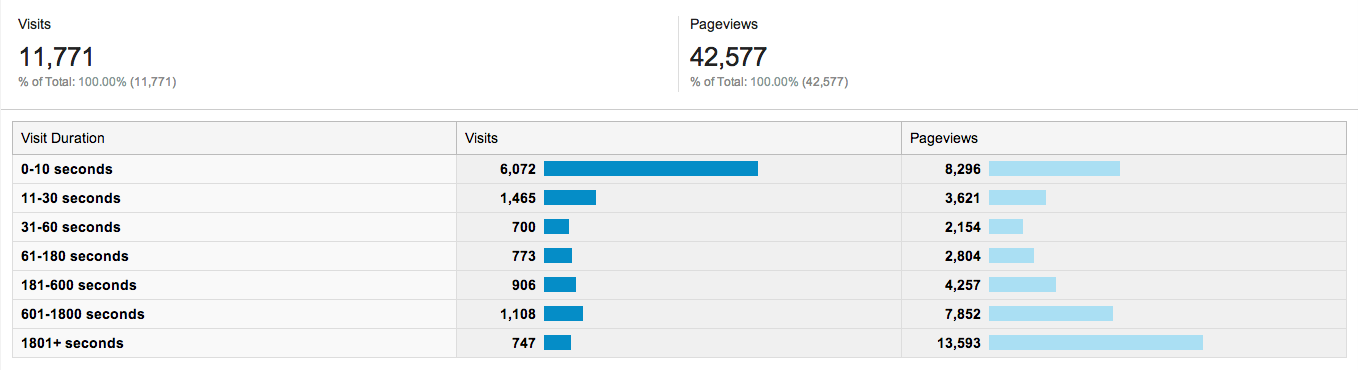
\includegraphics[trim= 0mm 0mm 0mm 0mm, clip, scale=0.3]{./Figures/UserStratificationVisitLength}
\caption{User Engagement by Visit Length}
\label{fig:UserStratificationVisitLength}
\end{figure}

This user stratification into extremely high and extremely low involvement raises the issue of user saturation: people were either hooked and used the site very frequently or they used it a few times and left. As a result, the user base contained a small number of power-users and a large number of amateur-users who visited the site infrequently at best. This most likely resulted in a poor user experience for both classes of users. The amateur-users may not have become acclimated to the norms of anonymous conversation and might be intimidated by a conversation with a power-user, but they might bored with a conversation with another amateur-user. Conversely, a power-user would be used to the norms of an anonymous conversation, and would likely get bored conversing with amateur-user. This is because most amateur- users would still likely be operating under normal conversational norms, which the power-users would be trying to escape. Although a power-user would enjoy talking to another power-user, he or she would quickly run out of new power-users to talk to.

The solution to this problem is to have a `casual user': a user who visits TA on a regular basis but not frequently enough to be considered a power-user. These `casual users' would be familiar with the norms of anonymous conversation and would provide new conversational partners for power-users while still enjoying the occasional conversation with an amateur-user. In this way, they would bridge the gap between the two previous user categories and provide a better TA experience for all. 

It is for this reason that I am currently working on a new project, named Campus Anonymous, which will be released to all the universities in the Ivy League. This new website will have access to a broader user base than TA and thus increase the likelihood of attracting a non-trivial set of `casual users'.
